%% LyX 2.3.0 created this file.  For more info, see http://www.lyx.org/.
%% Do not edit unless you really know what you are doing.
\documentclass[12pt,english]{article}
\usepackage{mathptmx}
\renewcommand{\familydefault}{\rmdefault}
\usepackage[T1]{fontenc}
\usepackage[latin9]{inputenc}
\usepackage{geometry}
\geometry{verbose,tmargin=2cm,bmargin=2cm,lmargin=2cm,rmargin=2cm}
\usepackage{float}
\usepackage{graphicx}

\makeatletter
%%%%%%%%%%%%%%%%%%%%%%%%%%%%%% User specified LaTeX commands.
\usepackage{lineno} 
\linenumbers


\usepackage{xr}
\externaldocument{coexistence_species-rich}

\makeatother

\usepackage{babel}
\begin{document}
\emph{Electronic Supplementary Material} to \textbf{How self-regulation, the storage effect and their interaction contribute to coexistence in stochastic and seasonal environments}. Picoche,~C. \& Barraquand,~F.

\appendix

\section{Biomass-trait distributions} %Was before supplementary figures

\renewcommand\thefigure{\thesection.\arabic{figure}} 

\begin{figure}[H]
\begin{centering}
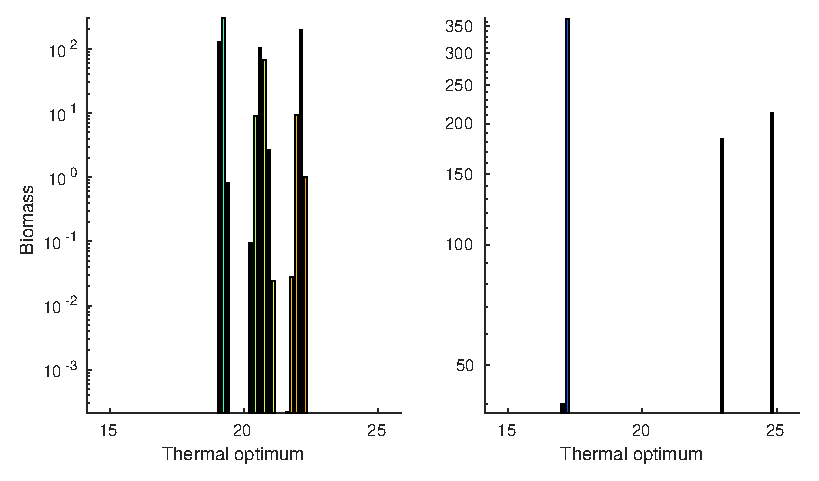
\includegraphics[width=0.95\textwidth]{graphe/FigS1}
\par\end{centering}
\caption{Temporal mean of biomass as a function of the thermal optimum defining
each species. The temporal means are computed over the last 200 years
of a simulation spanning 5000 years. We considered both a random
(left) and a seasonal signal for the temperature (right). The coexistence mechanism
implemented is the storage effect, and the intra and interspecific competition coefficients are equal. This
simulation is the one described in Fig. 1
in the main text\label{fig:Appendix_mean_biomass_iter2}. 99 other simulations
have been performed to produce the main text results in Figs. 2-4. }
\end{figure}

\begin{figure}[H]
\begin{centering}
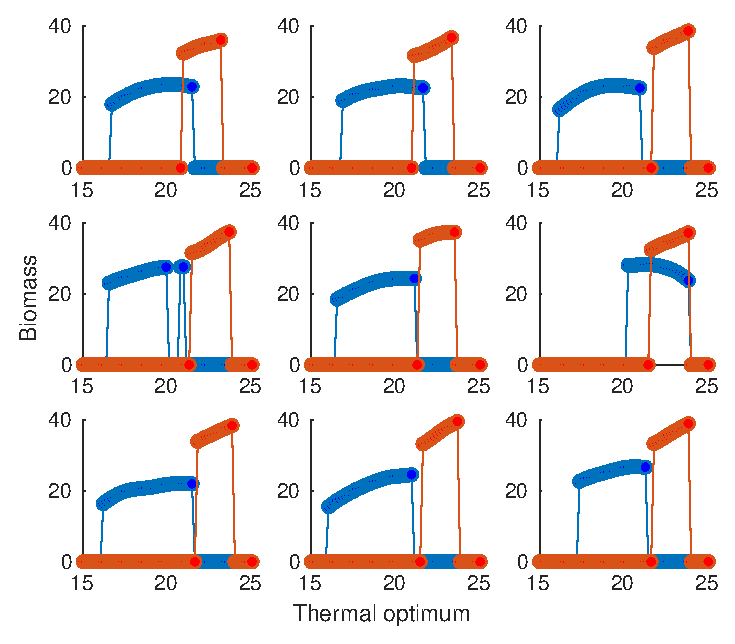
\includegraphics[width=0.95\textwidth]{graphe/example_iteration}
\par\end{centering}
\caption{Temporal mean biomass distribution, computed over the last 200 years,
for 9 representative simulations, as a function of the thermal optimum
of the species. These simulations are done without storage effect
but with a strong self-regulation. Temperature is either a seasonal
signal (red) or a random noise (blue). The distribution induced
by a random noise overlaps the one obtained with a seasonal noise in only 2 simulations out of 100, hence the 2 signals
lead in general to non-overlapping biomass distributions on the
trait axis. \label{fig:Not_representative_behaviour} }
\end{figure}

\section{Variation in mortality rates}
\setcounter{figure}{0}
To test the robustness of our conclusions while accelerating convergence, we conducted the same analyses with a species-specific mortality rate. For each set of simulations, covering 4 different competition scenarios and 2 types of environmental forcing, the mortality rate was drawn from a uniform distribution between 14.9 and 15.1 year$^{-1}$ so that we only changed the variability, but not the mean, of this parameter. 

The main results of our analyses were not altered by this modification (Fig. \ref{fig:Nb_extant_morta_variable}). The absence of coexistence mechanisms led to competitive exclusion of all species but one and the presence of both coexistence mechanisms maintained all species (Fig. \ref{fig:Fig3_morta_variable}). Strong self-regulation on its own maintained between 23 and 31 species (vs 20 to 32 in the case of constant mortality) with a random noise, and between 12 and 14 (vs 12 to 15 with a constant mortality) with a seasonal noise. The storage effect alone also led to similar results with a seasonal noise with regards to the richness of the community. As shown on Fig. \ref{fig:Fig4_morta_variable}, biomass-trait distributions remained qualitatively similar (multimodality with the storage effect and uniform distribution with a strong self-regulation, with different partitioning on the trait axis depending on the type of noise). The only case which led to slightly different results was the combination of a storage effect and random noise. In this case, the final number of species in the community ranged from 2 to 6, with nearly 50\% of the simulations ending with 3 species only. Richness is therefore approximately 4 times lower than what was obtained with a constant mortality. The remaining species had approximately the same positions on the trait axis as in the case of a constant mortality. 

\begin{figure}[H]
\begin{centering}
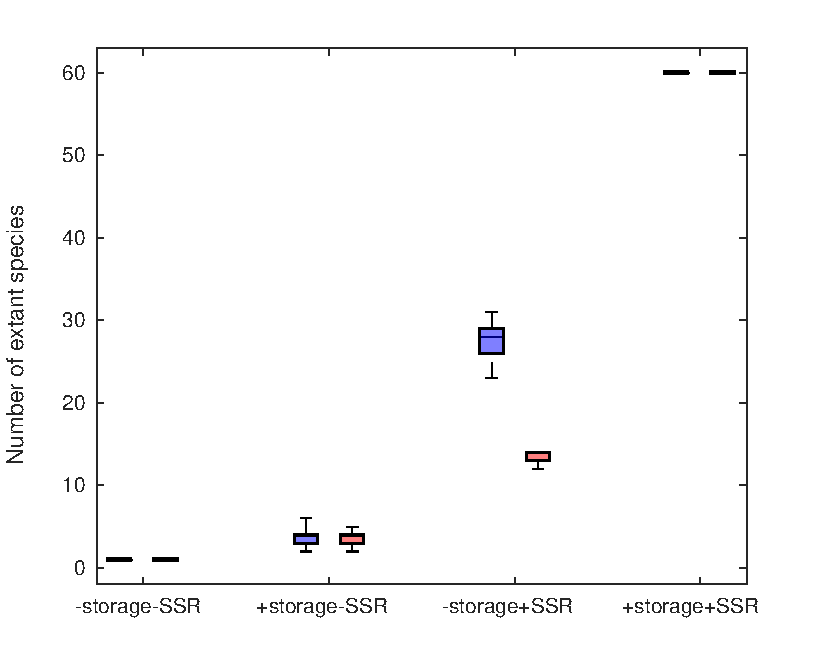
\includegraphics[width=0.75\textwidth]{graphe/Fig2_mortavariable}
\par\end{centering}
\caption{Number of species still present at the end of 100 simulations (5000 years each) with a variable mortality,
initialized with 60 species, with a random forcing signal (blue) or a seasonal noise (red). The
signs + or -storage refer to presence or absence of the storage effect, respectively; + / - SSR,
presence or absence of Strong Self-Regulation, respectively. Community compositions are stable
in the cases -storage-SSR and +storage+SSR, for which 1 or 60 species are still present at the
end of all simulations. Due to low variance, the whiskers here represent min and
max rather than 1.5 interquartile range.\label{fig:Nb_extant_morta_variable}}
\end{figure}

Competitive exclusion within clumps was therefore accelerated by the variation in mortality. This can be explained by the departure from neutral dynamics which, in the absence of immigration, led to the exclusion of species being even marginally more vulnerable than the others within their clumps. We can assume that the results obtained with a variable mortality mimic the ones that could be obtained with a constant mortality but for much longer runtimes, after the longest transients. 

\begin{figure}[H]
\begin{centering}
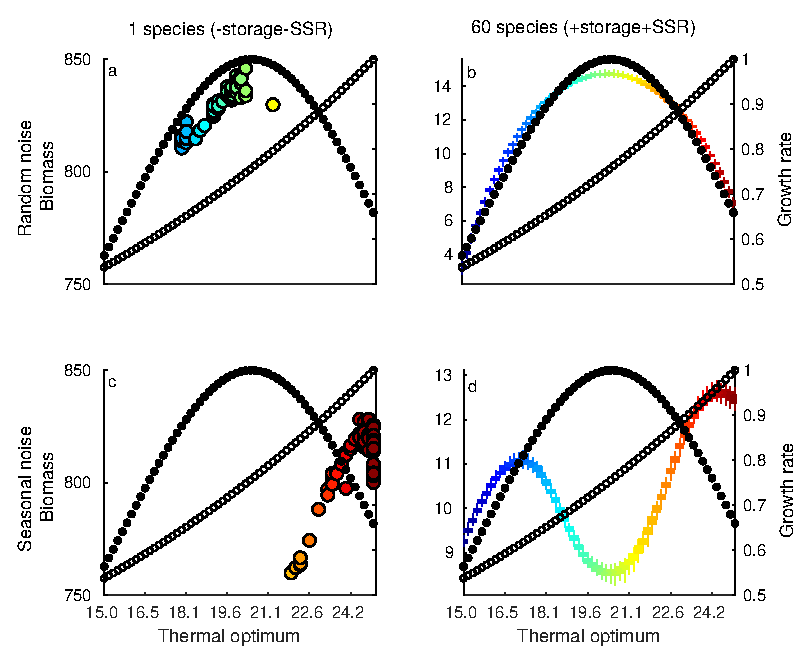
\includegraphics[width=0.75\textwidth]{graphe/Fig3_morta_variable}
\par\end{centering}
\caption{Mean biomass distribution over the last 200 years for 100 simulations, as a function of the species thermal optima. 
We consider here a variable mortality between species. Here we consider the
two stable-composition cases and two types of forcing signal. On the
left column, simulations without storage effect nor strong self-regulation
are presented. Only one species is present at the end of the simulations
and its mean value is represented by one large colored circle per
simulation. There can be several circles for the same species, corresponding
to multiple simulations ending with this species alone. On the right
column, simulations with storage effect and strong self-regulation
are represented. All species are present at the end of the simulations
and small boxplots present the variation in the temporal average of
biomass with a given trait, for 100 simulations. The forcing signal
is either a random (top) or a seasonal noise (bottom). Each species
is identified by its thermal optimum through its color code. Scaled
(divided by maximum) average and maximum growth rates are shown as
small filled and open circles, respectively, and are indexed on the
right y-axis.\label{fig:Fig3_morta_variable}}
\end{figure}

\begin{figure}[H]
\begin{centering}
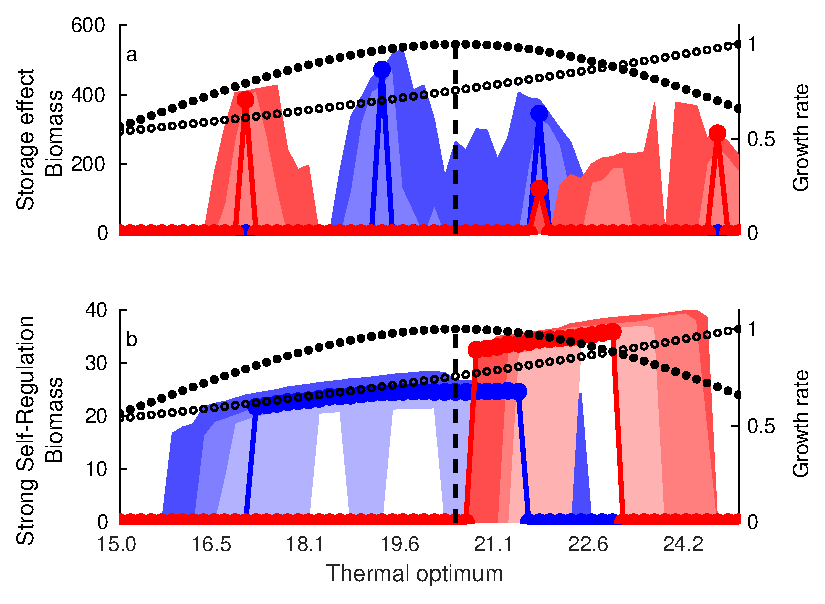
\includegraphics[width=0.75\textwidth]{graphe/Fig4_morta_variable}
\par\end{centering}
\caption{Mean biomass distribution over the last 200 years for 100 simulations as a function of thermal optima. 
We consider here a variable mortality between species. The two cases considered are (a) with storage effect and equal competitive
strengths and (b) without storage effect, with strong self-regulation. The forcing signal is either a random (in blue) or a seasonal
noise (in red). Shades of the same color correspond to the 50th, 90th and 100th percentiles of the distributions while colored lines correspond
to one representative simulation. Scaled (divided by maximum) average (whose maximum is indicated by the dashed line) and maximum growth
rates are shown as filled and open and circles, respectively, and indexed on the right y-axis.\label{fig:Fig4_morta_variable}}
\end{figure}

\end{document}
